\documentclass[12pt]{article}

\usepackage[margin=1 in]{geometry}

%Use Times New Roman font
%\usepackage{pslatex}

% allow text colors
\usepackage[usenames,dvipsnames,svgnames,table,x11names]{xcolor}

%allow double-spacing
\usepackage{setspace}

%enable support for figures
\usepackage{graphicx}

\usepackage{rotating}
\usepackage{multirow}

\usepackage{url}

%handle filenames better
\usepackage{grffile}

%math
%\usepackage{mathtools}
\usepackage{amsmath}
\usepackage{amsfonts}
\usepackage{lipsum}

%control figure movement
\usepackage{placeins}

%center captions
\usepackage{caption}

%circuits and units
\usepackage[free-standing-units]{siunitx}
\DeclareSIUnit\vrms{\volt{}_{RMS}}
%\usepackage[americanvoltages,americancurrents]{circuitikz}
%\usetikzlibrary{calc}

% make scientific notation easy
\providecommand{\e}[1]{\ensuremath{\times 10^{#1}}}

% include pdf documents
\usepackage{pdfpages}

%for loops
\usepackage{pgffor}

%indent after new sections
\usepackage{indentfirst}

\usepackage{verbatim}

% allow greek letters outside math mode. \text<name of letter>
%\usepackage{textgreek}

% margin editing
\usepackage{changepage}

% braket notation, other goodies
\usepackage{physics}
\usepackage{braket}

%source code
\usepackage{listings}

%hyperlink support
\usepackage{hyperref}

% bibtex support
\usepackage{natbib}

%settings for Python code
%\lstset{basicstyle=\footnotesize\ttfamily,
%commentstyle=\color{OliveGreen},
%keywordstyle=\color{blue},
%tabsize=4,
%numbers=left,
%stringstyle=\color{red},
%language=Python,
%inputencoding=utf8,
%extendedchars=true,
%showstringspaces=flase,
% }

\begin{document}
\singlespacing
\title{Final Report\\
AST 383}
\date{Dec 15 2015}
\author{Robert Rosati \\ Mar\'{i}a Jos\'{e} Bustamante Rosell}
\maketitle

\begin{abstract}
\par Blah blah blah. Clusters are pretty man.
\end{abstract}

\doublespacing
\section{Motivation}

\section{Clustering Algorithms}
\par We decided to survey a few clustering algorithms.
\texttt{DBSCAN} is quite similar to Rockstar's algorithm, so it was a natural choice.
One paper we saw in class \cite{FIDEPE}, described a new density-based algorithm that we thought could potentially give better performance, or at the very least more fully survey the landscape of clustering algorithms.

\subsection{\texttt{DBSCAN}}
\begin{figure}[ht]
\centering
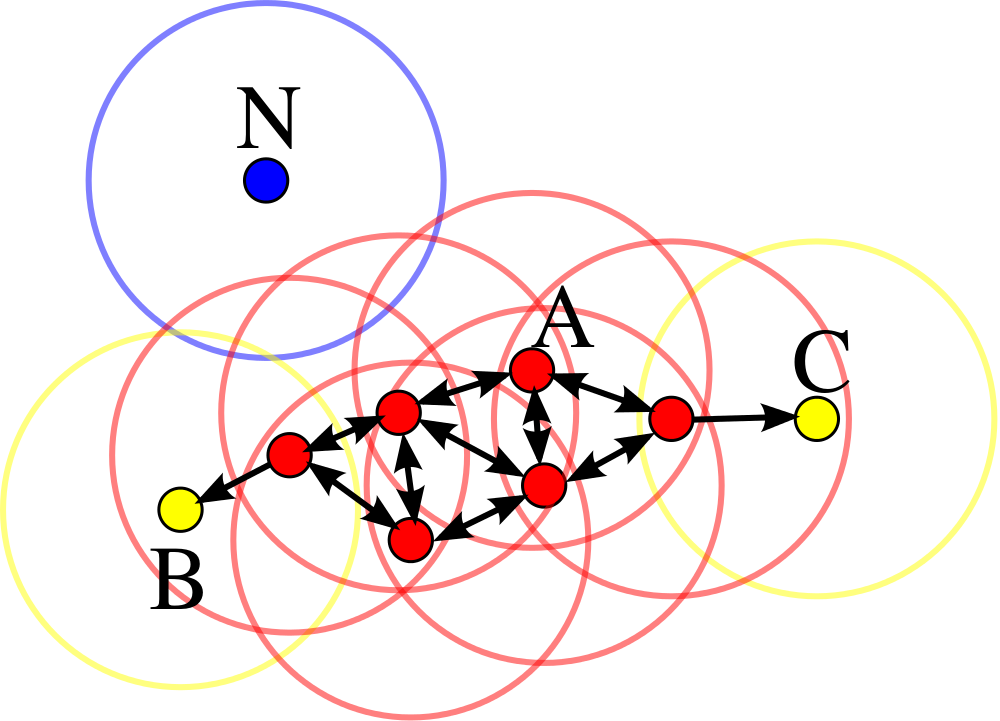
\includegraphics[width=0.8\linewidth]{DBSCAN-Illustration}
\caption{How \texttt{DBSCAN} selects the points in a cluster.}
\label{fig:DBSCAN}
\end{figure}


% when talking about code
\par It's worth noting a few optimizations that can be made to this algorithm.
The distances between points, instead of being computed for each point ($O(N^2)$ lookups), can be computed in a type of tree structure ($O(N \log(N))$ lookups). Such position-tree structures are often called R-trees or R*-trees.
In addition, the \texttt{expandCluster} routine is only called from a single location, so it may be safely inlined.

%prediction under varying parameters

\subsection{FIDEPE}

\texttt{FIDEPE} (FInd DEnsity PEaks) algorithm \cite{FIDEPE} considers two criteria per point: Local Density and Minimum Distance to a point of higher density.

Local density ($\boldsymbol{\rho}$), is defined as the number of points $j$ in the "neighborbood"; points closer than $d_c$ from point $i$.
\begin{align*}
	\rho_i = \sum_j \chi(d_{ij}-d_c)
\end{align*}
where 
\begin{align*}
\chi(x)=
\begin{cases}
1 & x < 0 \\
0 & otherwise
\end{cases}
\end{align*}

Minimum Distance to a point of higher density (\textbf{Delta}) is self explanatory. 

\begin{align*}
	\delta_i = \text{min}_{j:\rho_j > \rho_i} (d_{ij})
\end{align*}

For the point of highest density though, \textbf{Delta} is just the maximum distance to another point.

\begin{align*}
	\delta_i = \text{max}_{j} (d_{ij})
\end{align*}

\begin{figure}[ht]
\centering
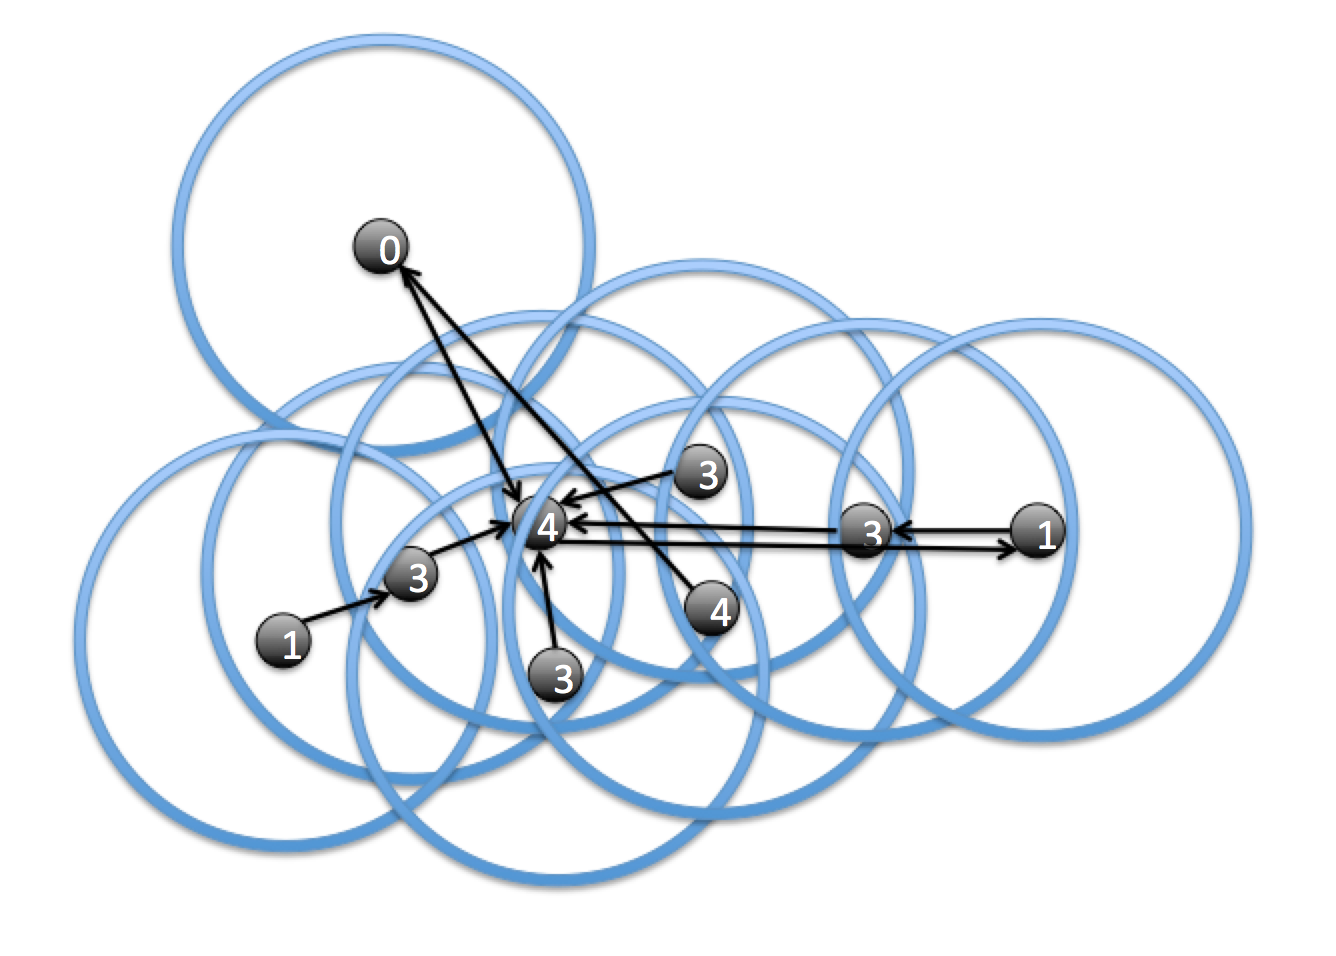
\includegraphics[width=0.8\linewidth]{fidepe_plots/FIDEPE}
\caption{How the \texttt{FIDEPE} algorithm identifies points in a cluster.}
\label{fig:FIDEPE}
\end{figure}


Figure \ref{fig:FIDEPE} shows a simple example of the quantities above described. Here \textbf{Rho} is marked as numbers above each of the points, the circles around them define a neighborhood of radius $d_c$ and the directed arrows are \textbf{Delta}.


Once this two quantities are defined for each point the algorithm identifies the points with both the highest \textbf{$\rho$} and \textbf{$\delta$} and tags them as cluster centers. The choice for how many of them fall under this criterion is not specified in the original code. We decided to select points 5 $\sigma$ away from the mean for \textbf{$\delta$} and 1 $\sigma$ away for \textbf{$\rho$}. This proved far away from robust.

\section{Plots}

\begin{figure}[ht]
\centering
%\includegraphics[scale=0.8]{plots/D31}
\caption{Our reference distributions.}
\label{fig:reference}
\end{figure}

\begin{figure}[ht]
\centering
\raisebox{0.75in}{\rotatebox[]{90}{Aggregation}}
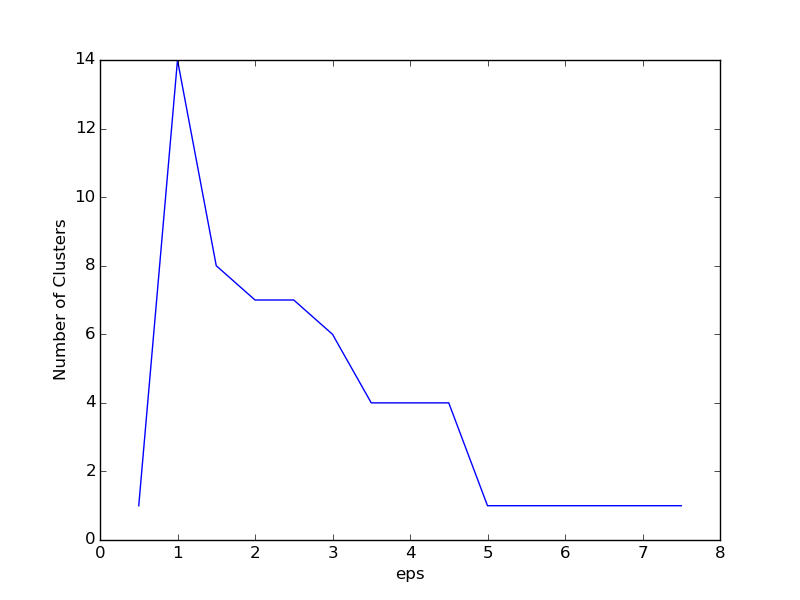
\includegraphics[width=0.35\linewidth]{plots/Aggregation_eps} 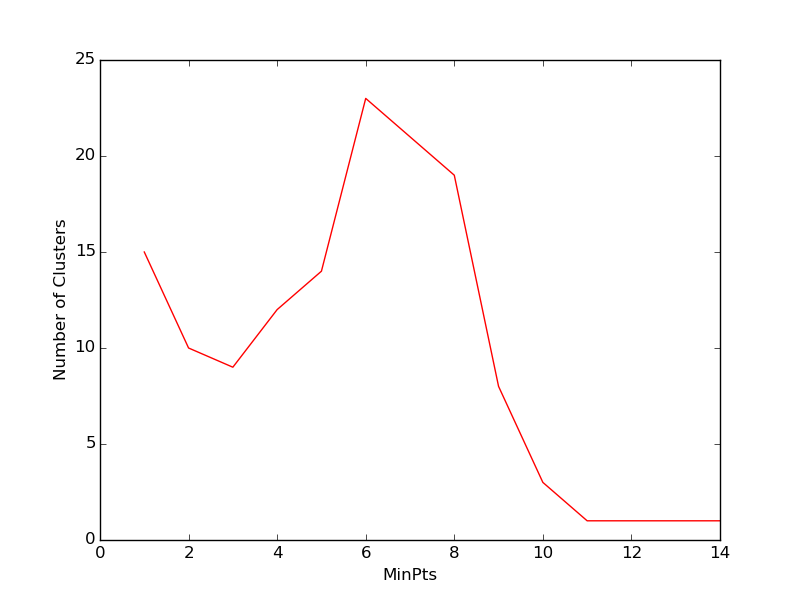
\includegraphics[width=0.35\linewidth]{plots/Aggregation_minpts} \\
\raisebox{0.75in}{\rotatebox[]{90}{Compound}}
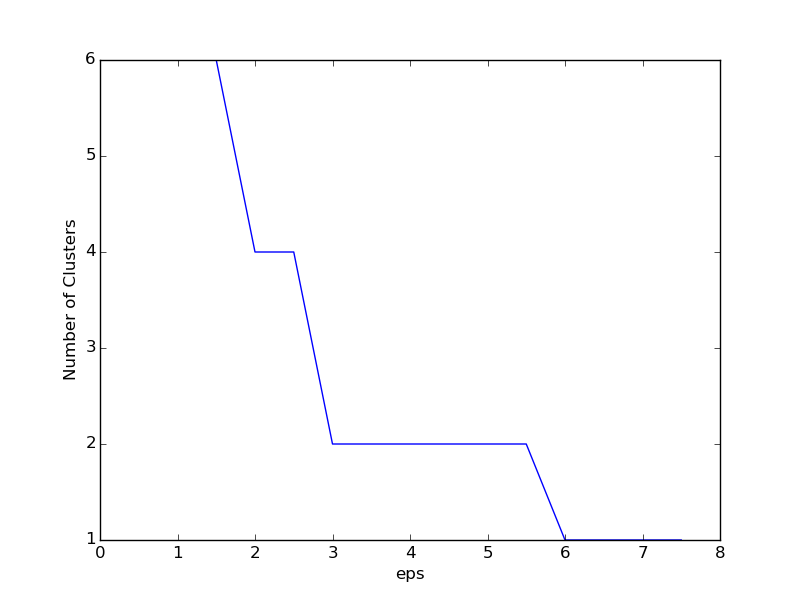
\includegraphics[width=0.35\linewidth]{plots/Compound_eps} 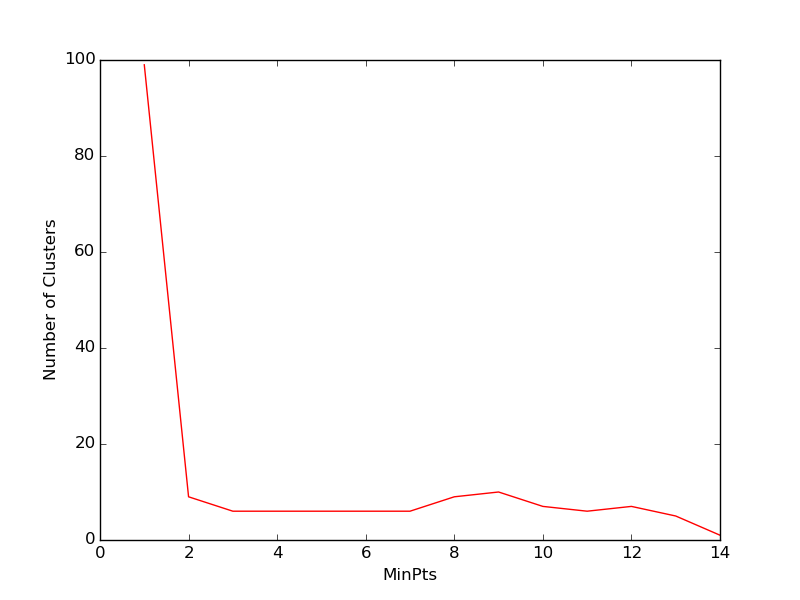
\includegraphics[width=0.35\linewidth]{plots/Compound_minpts} \\
\raisebox{0.75in}{\rotatebox[]{90}{D31}}
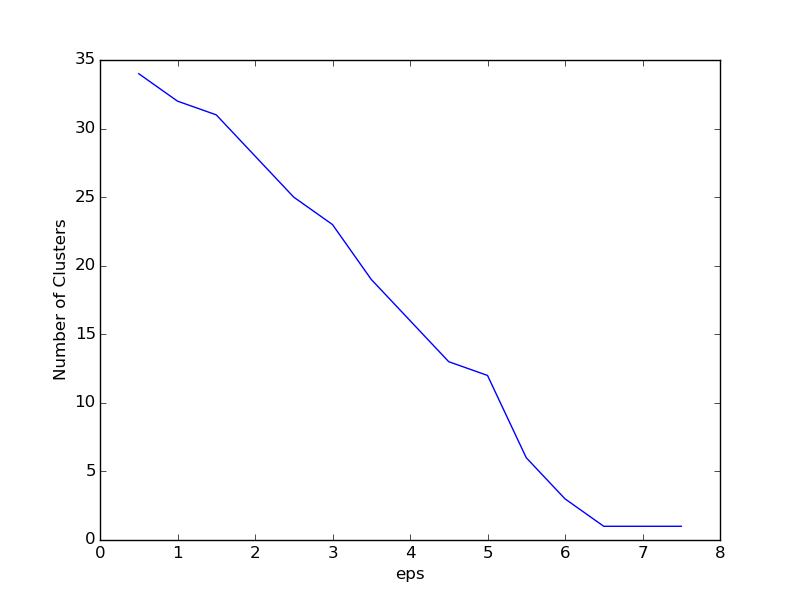
\includegraphics[width=0.35\linewidth]{plots/D31_eps}
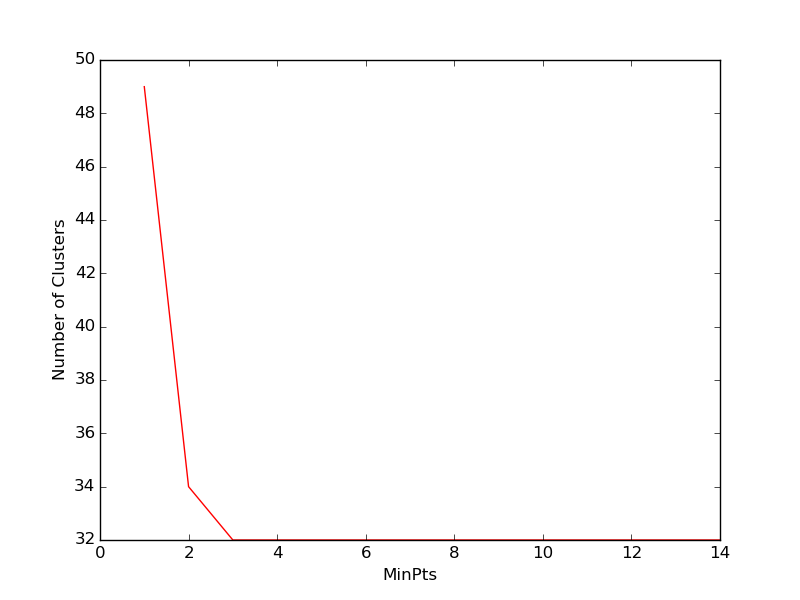
\includegraphics[width=0.35\linewidth]{plots/D31_minpts} \\
\raisebox{0.75in}{\rotatebox[]{90}{jain}}
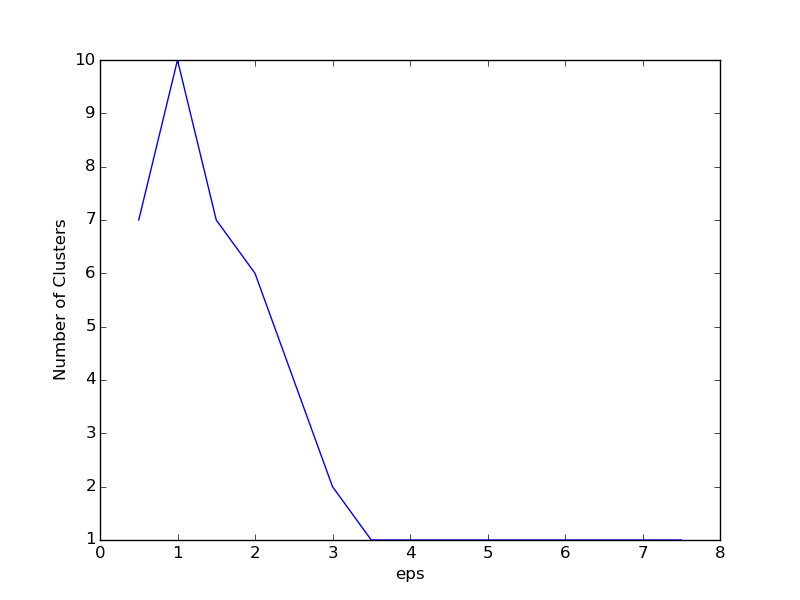
\includegraphics[width=0.35\linewidth]{plots/jain_eps}
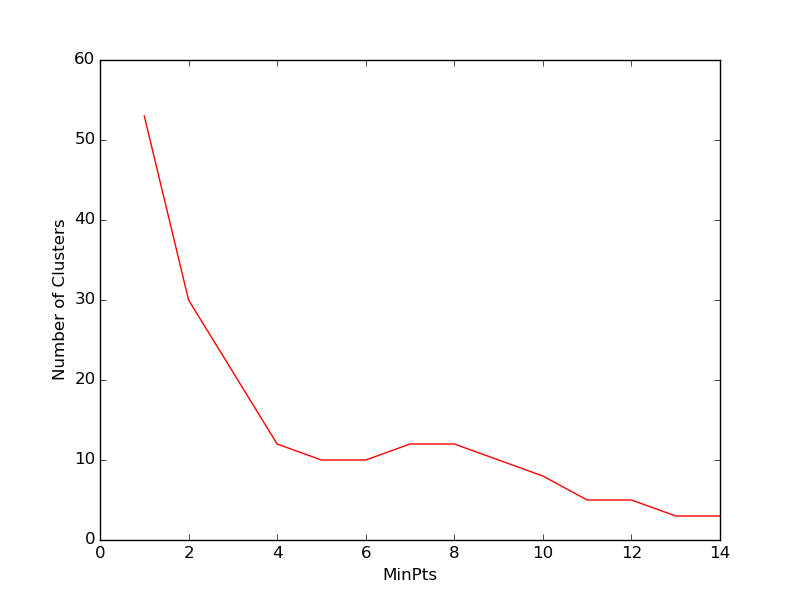
\includegraphics[width=0.35\linewidth]{plots/jain_minpts} \\
\raisebox{0.75in}{\rotatebox[]{90}{spiral}}
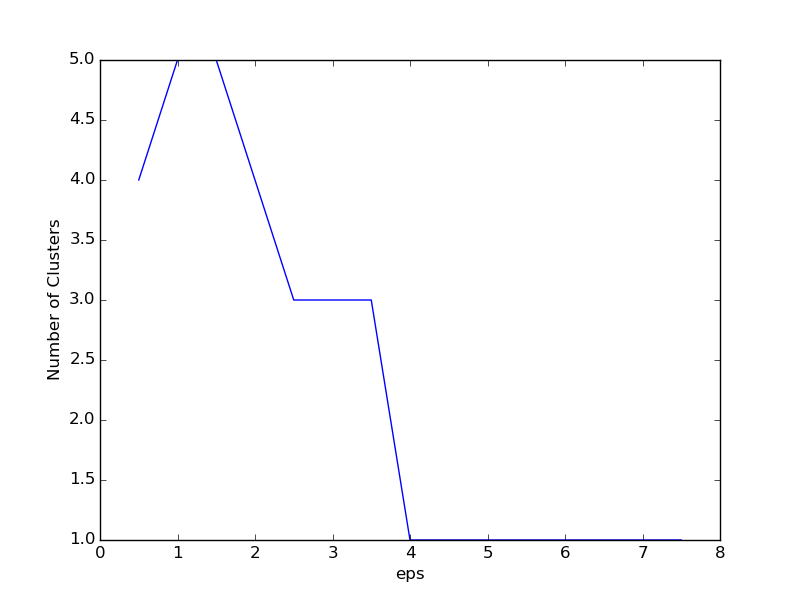
\includegraphics[width=0.35\linewidth]{plots/spiral_eps}
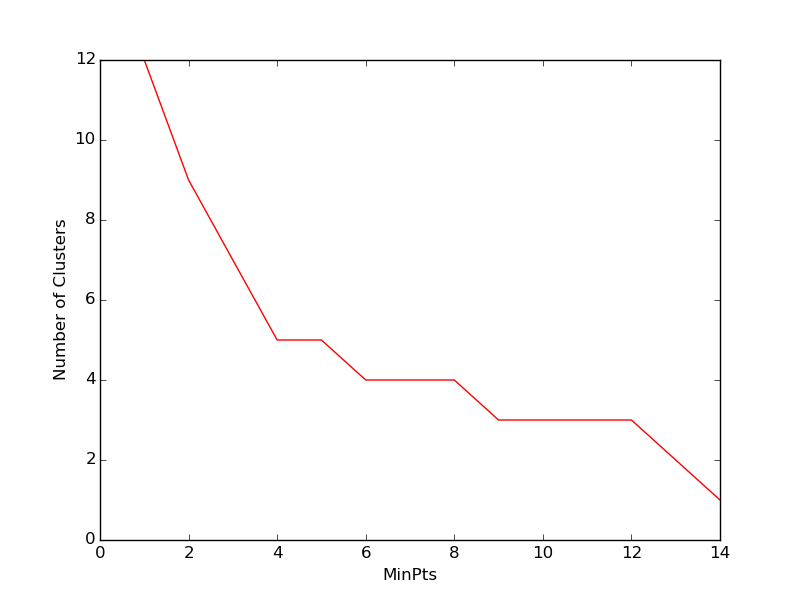
\includegraphics[width=0.35\linewidth]{plots/spiral_minpts}
\caption{(Left) The effects of varying the \texttt{eps} parameter of \texttt{DBSCAN} for all reference distributions. \\ 
(Right) The effects of varying the \texttt{MinPts} parameter of \texttt{DBSCAN}}.
\label{fig:DBSCANplots}
\end{figure}


\begin{figure}[ht]
\centering

\caption{The effects of varying the \texttt{FIDEPE} parameters.}
\label{fig:FIDPEPEplots}
\end{figure}


\section{Results}
\par Referencing Figure \ref{fig:DBSCANplots}, the \texttt{DBSCAN} algorithm does not seem particularly robust to variation in either \texttt{eps} or \texttt{MinPts}. Our proposed mechanism for objectively identifying the number of active clusters appears to fail in almost all test cases. The \texttt{spiral} dataset seems to be the exception, in that the flattest regions of the plots occur at the true number of clusters. The most densely clustered dataset, \texttt{D31}, converges in the range of \texttt{MinPts} plotted to the true cluster number, but fails to plateau in the range of \texttt{eps} plotted. (Describe other datasets?)
\par Our choice not to explore the full parameter space for these plots likely has contributed to our inability to find the peak cluster plateau we na\"\i vely expect. However, there is no guarantee of any sort of robustness in these algorithms. It may possible to construct datasets with a plateau on a false cluster number somewhere in the parameter space. We leave these questions for future work, now only concluding that is heuristic is useful in some nonzero percentage of typical datasets.
\clearpage
\bibliographystyle{plain}
\bibliography{research}

\end{document}
